%%%%%%%%%%%%%%%%%%%%%%%%%%%%%
%% Styles, packages and new commands
\input{../Main/ML_Main.tex}
%%%%%%%%%%%%%%%%%%%%%%%%%%%%%
%% Edit the title page
\title{Machine Learning}
\subtitle{Module 6: Ensemble methods}
\author[MOB]{Marc-Olivier Boldi}
\institute[HEC MSc Mgt BA]{Master in Management, Business Analytics, HEC UNIL}
\date[Spring 2024]{Spring 2024}
%%%%%%%%%%%%%%%%%%%%%%%%%%%%%
%%%%%%%%%%%%%%%%%%%%%%%%%%%%%
%%%%%%%%%%%%%%%%%%%%%%%%%%%%%
%%%%%%%%%%%%%%%%%%%%%%%%%%%%%
\begin{document}
%%%%%%%%%%%%%%%%%%%%%%%%%%%%%
\begin{frame}
  \titlepage
\end{frame}
%%%%%%%%%%%%%%%%%%%%%%%%%%%%%
\begin{frame}
\frametitle{Table of Contents}
	\tableofcontents
\end{frame}
%%%%%%%%%%%%%%%%%%%%%%%%%%%%%
\section{Ensemble and bagging}
%%%%%%%%%%%%%%%%%%%%%%%%%%%%%
\begin{frame}
\frametitle{Ensemble}
Until now we have tried to train the best learner among several candidates to solve a given task. \\
\vspace{0.2cm}
On the contrary, an {\bf ensemble} learner is made of several learners (so called {\bf base learners} or {\bf sub-learners}) that are combined for the prediction. \\
\vspace{0.2cm}
Base learners are often simple learners, coming from an homogenous family of learners (e.g. regression trees, regressions, etc.). 
\end{frame}
%%%%%%%%%%%%%%%%%%%%%%%%%%%%%
\begin{frame}
\frametitle{Bagging}
{\bf Bagging} stands for {\bf Bootstrap AGGregatING}. It is a way to build an ensemble learner from several versions of the same learner, trained on bootstrapped versions of the same training set: 
\begin{itemize}
\item Draw several random samples (with replacement) from the training data set, 
\item For each sample, construct a separate model and separate predictions for your test set.
\item Averaged these predictions to create a final prediction value.
\end{itemize}
The objective of the intensive randomization is to built many small {\it uncorrelated} learners rather than one unique big learner.
\end{frame}
%%%%%%%%%%%%%%%%%%%%%%%%%%%%%
\begin{frame}
\frametitle{Bagging}
\begin{center}
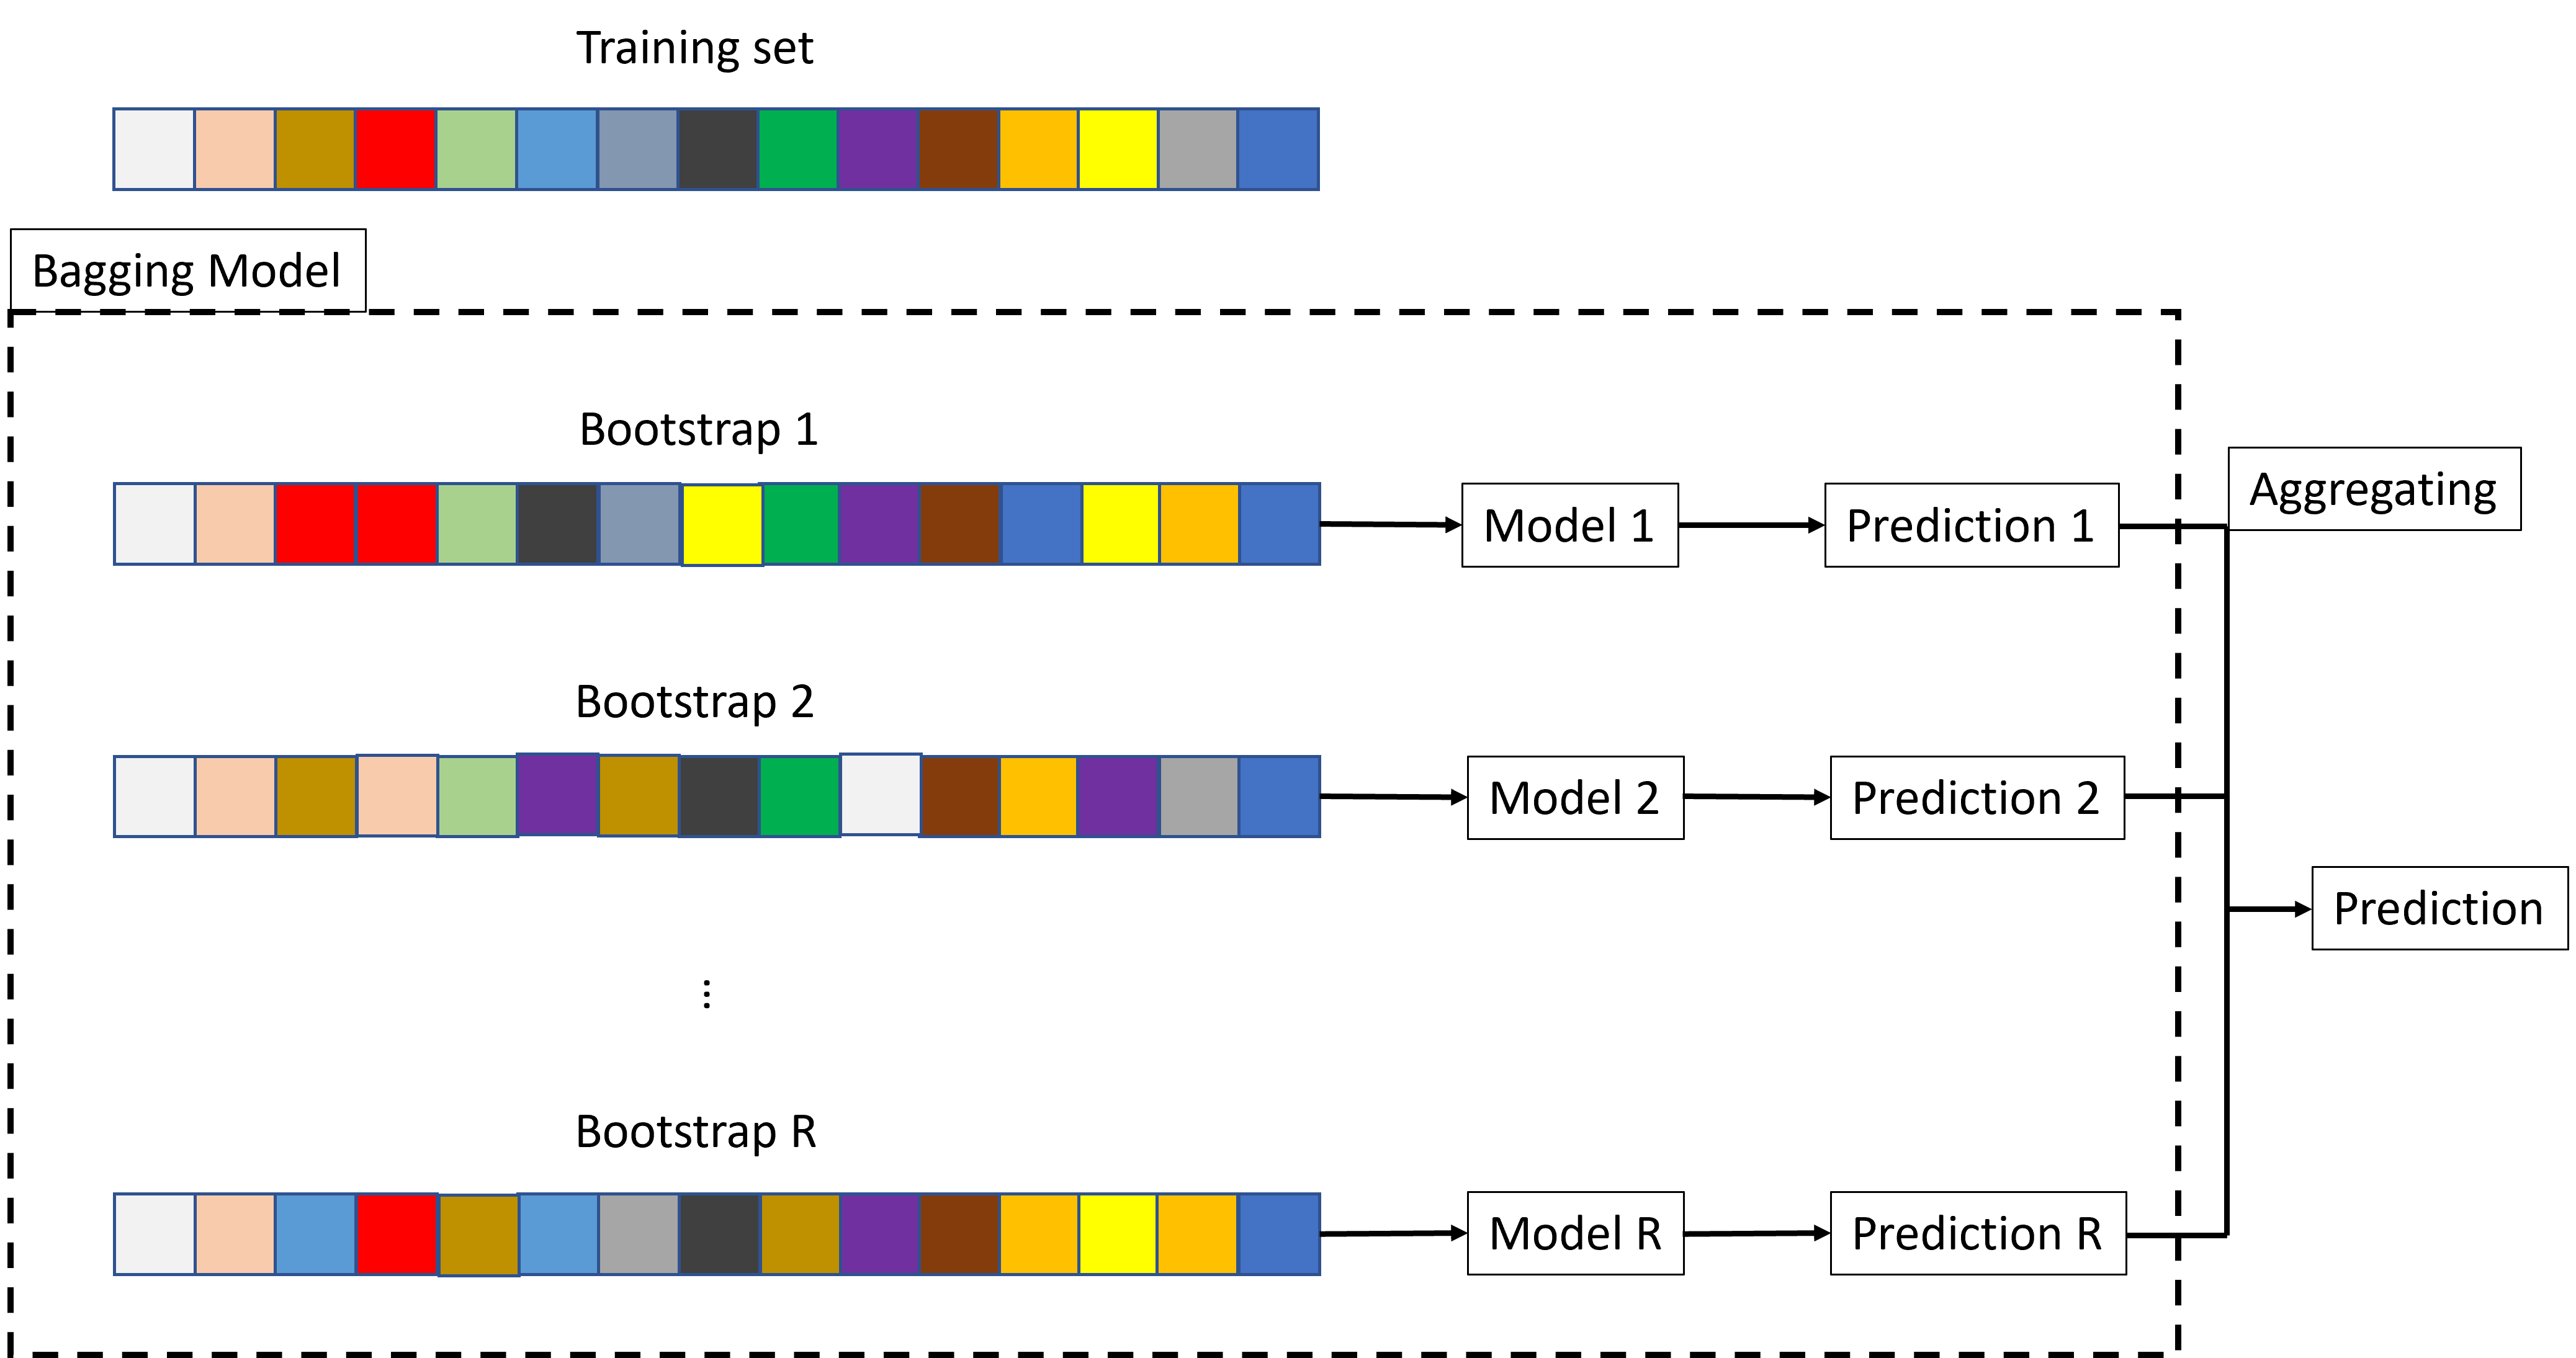
\includegraphics[width=12cm]{../Graphs/Bagging.png}
\end{center}
\end{frame}
%%%%%%%%%%%%%%%%%%%%%%%%%%%%%
\begin{frame}
\frametitle{Bagging}
Does it work and why? (in theory...)
\begin{itemize}
\item Overfitting: no model is trained on the whole training set. Thus, no model can overfit it.
\item Accuracy: each resampled data set is similar to the training set. Thus, it can produce the same accuracy as the one trained on the whole training set.
\end{itemize}
Thus, in theory, there is no reason why each model has a lower accuracy than a model that would be trained on the whole training set.\\
\vspace{0.3cm}
In addition, there is no reason why they, together, could overfit the training set since no model can overfit it.
\end{frame}
%%%%%%%%%%%%%%%%%%%%%%%%%%%%%
\begin{frame}
\frametitle{Bagging}
In practice, bagging is efficient when the features are unstable and very influential on the model (e.g., outliers).\\
\vspace{0.3cm}
The properties of bagging come at the cost of extra complexity: 
\begin{itemize}
\item A {\bf large number of models} must be kept in memory to make the final prediction.
\item Even if each model are interpretable (e.g., regressions), the final model is {\bf not interpretable}.
\end{itemize}
However, unlike with a single model, the increase in complexity is {\bf not at the cost of over-fitting}. 
\end{frame}
%%%%%%%%%%%%%%%%%%%%%%%%%%%%%
\begin{frame}
\frametitle{Bagging}
When doesn't it work / how to improve it?
\begin{itemize}
\item If, bad luck, all the sub-models are similar $\rightarrow$ highly correlated.
\item The final model is no more than one of the sub-models.
\item It may overfit the training set and be poor in prediction (highly variable).
\end{itemize}
This may happen when the resampling has little effect. It is important that the sub-models are uncorrelated (or even independent) $\rightarrow$ random forest.
\end{frame}
%%%%%%%%%%%%%%%%%%%%%%%%%%%%%
%%%%%%%%%%%%%%%%%%%%%%%%%%%%%
%%%%%%%%%%%%%%%%%%%%%%%%%%%%%
\section{Random forest}
%%%%%%%%%%%%%%%%%%%%%%%%%%%%%
%%%%%%%%%%%%%%%%%%%%%%%%%%%%%
\begin{frame}
\frametitle{Concept}
{\bf Random forest} is a popular {\bf ensemble} method consisting of building lots of trees whose predictions will be averaged to produce one final prediction. In practice: 
\begin{enumerate}
\item Draw at random $M$ subsets from the training set: same size as the original one, with replacement. 
\item On each subset, grow a small tree with: at each split trial, a small amount of features is drawn at random: you have $M$ small trees.
\item The RF prediction is the average of the $M$ trees for regression, or the vote majority for classification.\\
\end{enumerate}
Point 1. is bagging. Point 2 is an additional mixing technique to enhance sub-model non-correlation.
\end{frame}
%%%%%%%%%%%%%%%%%%%%%%%%%%%%%
\begin{frame}
\frametitle{Why does that work?}
The reasons are the same as for bagging.\\
\vspace{0.3cm} 
Furthermore, with the additional mixing of the features when constructing the trees:
\begin{itemize}
\item each tree remains unbiased (it has the same chance to get the best features).
\item the trees are even less correlated than with bagging alone. This brings more stability.
\end{itemize}
\end{frame}
%%%%%%%%%%%%%%%%%%%%%%%%%%%%%
\begin{frame}
\frametitle{Variants}
There exist several variants of RF. Below, some default settings of {\tt randomForest} function:
\begin{itemize}
\item If the re-sampling is with replacement, then the subset is of the same size as the training set.
\item If the re-sampling is without replacement, then the subset is of size 0.632 of the training set . 
\item The number of features at each split is $\sqrt{p}$ for classification and $p/3$ for regression. 
\end{itemize}
\end{frame}
%%%%%%%%%%%%%%%%%%%%%%%%%%%%%
\begin{frame}
\frametitle{Variants}
More {\bf hyperparameters} of {\tt randomForest}:
\begin{itemize}
\item Number of trees: ${\tt ntrees} = 500$
\item Number of variables: ${\tt mtry}$ is the number of features selected at random; $\sqrt{p}$ for classification and $p/3$ for regression.
\item Sample size: {\tt sampsize} same as the data set (training set) when {\tt replace=TRUE}, and 0.632 of {\tt sampsize} when {\tt replace=FALSE}.
\item Maximum tree size: {\tt maxnodes} as large as possible, can be set.
\item Maximum node size: {\tt nodesize} 1 for classification and 5 for regression.
\end{itemize}
These hyperparameters can be tuned.
\end{frame}
%%%%%%%%%%%%%%%%%%%%%%%%%%%%%
\begin{frame}
\frametitle{Final words}
\begin{itemize}
\item Random forest is an ensemble method that combines bagging and feature mixing.
\item It is often a good learner: good fit, not prompt to overfitting.
\item It may be not better than a single model (e.g., a tree). 
\item It is not interpretable (no tree, coefficients, etc.).
\end{itemize}
\end{frame}
%%%%%%%%%%%%%%%%%%%%%%%%%%%%%
%%%%%%%%%%%%%%%%%%%%%%%%%%%%%
\section{Boosting}
%%%%%%%%%%%%%%%%%%%%%%%%%%%%%
%%%%%%%%%%%%%%%%%%%%%%%%%%%%%
\begin{frame}
\frametitle{Concept}
Unlike bagging that creates models in parallel, {\bf boosting} is an ensemble technique that creates models sequentially. 
\begin{itemize}
\item $T$ models $f_t$ are trained one after the other, $t=1,\ldots,T$,
\item The final boosting model $F_T(x)$ aggregates all the models
$$
F_T(x) = \sum_{t=1}^T \alpha_t f_t(x),
$$
\item At each step $k$, the next model $f_{k+1}$ is trained by giving more importance to the instance that are incorrectly classified by the current boosting model $F_k=\sum_{t=1}^k \alpha_t f_t$.
\item The model weight $\alpha_t$ is associated with the overall quality of $f_t$ (the better the quality, the larger the weight).
\end{itemize} 
\end{frame}
%%%%%%%%%%%%%%%%%%%%%%%%%%%%%
\begin{frame}
\frametitle{Variations}
There exist lots of versions of the boosting:
\begin{itemize}
\item Usually, $f_t$ is a {\bf weak learner}: a simple learner, easy to train. It must be possible to assign a weight to each instance. E.g., a 1-split decision tree. 
\item In theory, one could boost any model.
\item The number of models, $T$ is arbitrary.
\item The computation of the instance weights at each step may vary.
\item The computation of the model weight at each step may vary.
\item There exist several formula of the total error of the model. 
\end{itemize} 
\end{frame}
%%%%%%%%%%%%%%%%%%%%%%%%%%%%%
\begin{frame}
\frametitle{Adaboost}
One of the first boosting model\footnote{Freund, Y and Schapire, R E (1997). "A decision-theoretic generalization of on-line learning and an application to boosting". Journal of Computer and System Sciences. 55: 119-139.}. 
\begin{itemize}
\item Binary classification: $y$ is $-1$ or $1$.
\item Exponential loss: 
$$
L(F_k) = \sum_{i=1}^N e^{-y_i F_k(x_i)}
$$
\item Next model: $f_{k+1}$ minimize $\sum_i 1_{\{y_i \neq f_{k+1}(x_i)\}} e^{-y_i F_{k}(x_i)}$.
\item Model weight: 
$$
\alpha_{k+1} = \frac{1}{2} \ln \left(\frac{\sum_i 1_{\{y_i \neq f_{k+1}(x_i)\}} e^{-y_i F_{k}(x_i)}}{\sum_i 1_{\{y_i = f_{k+1}(x_i)\}} e^{-y_i F_{k}(x_i)}}\right)
$$ 
\end{itemize}
\end{frame}
%%%%%%%%%%%%%%%%%%%%%%%%%%%%%
\begin{frame}
\frametitle{Gradient boosting: a descent method}
\small
\begin{itemize}
\item Current apparent loss (general)
$$
L(F_k) = \sum_{i=1}^N L(y_i, F_k(x_i)).
$$
\item Compute the pseudo-residual (gradient) 
$$
g_k = -\frac{\partial L(F_k)}{\partial F_k} = -\left\{L_2(y_i, F_k(x_i))\right\}_{i=1,N},
$$
where $L_2$ is the derivative of $L$ wrt its second argument.
\item Train the new weak learner $f_{k+1}$ on $g_k$ (i.e., on $\{x_i, g_{k,i}\}$).
\item Find the model weight
$$
\alpha_{k+1} = \arg\min_{\alpha} \sum_{i=1}^N L(y_i, F_k(x_i) + \alpha f_{k+1}(x_i)).
$$
\item Update $F_{k+1} = F_k + \alpha_{k+1} f_{k+1}$.
\end{itemize}
\normalsize
\end{frame}
%%%%%%%%%%%%%%%%%%%%%%%%%%%%%
\begin{frame}
\frametitle{Regularization}
Overfitting can occur quickly with boosting. One way to prevent it is to use regularization:
$$
F_{k+1} = F_{k} + \nu \alpha_{k+1} f_{k+1},
$$
where $\nu$ is a {\bf learning rate}, fixed by the user.
\begin{itemize}
\item If $\nu = 1$ then there is no regularization,
\item If $\nu = 0$ then the model never learns.
\end{itemize}
To some extent this is equivalent to choose a low $T$ (total number of models) to avoid overfitting.\\
\vspace{0.3cm}
The learning rate can be tuned.
\end{frame}
%%%%%%%%%%%%%%%%%%%%%%%%%%%%%
\begin{frame}
\frametitle{Stochastic gradient boosting}
The evaluation of the gradient can be costly (and useless) if $N$ is large. One can act by random batches of data.\\ 
\vspace{0.3cm}
At each step, only a proportion $0 < p \leq 1 $ of the training set is used. The batch set is selected at random.\\
\vspace{0.3cm}
Using random batches can also diminish the risk of overfitting since it takes more time for the model to see all the data set.
\end{frame}
%%%%%%%%%%%%%%%%%%%%%%%%%%%%%
\begin{frame}
\frametitle{Bagging vs boosting}
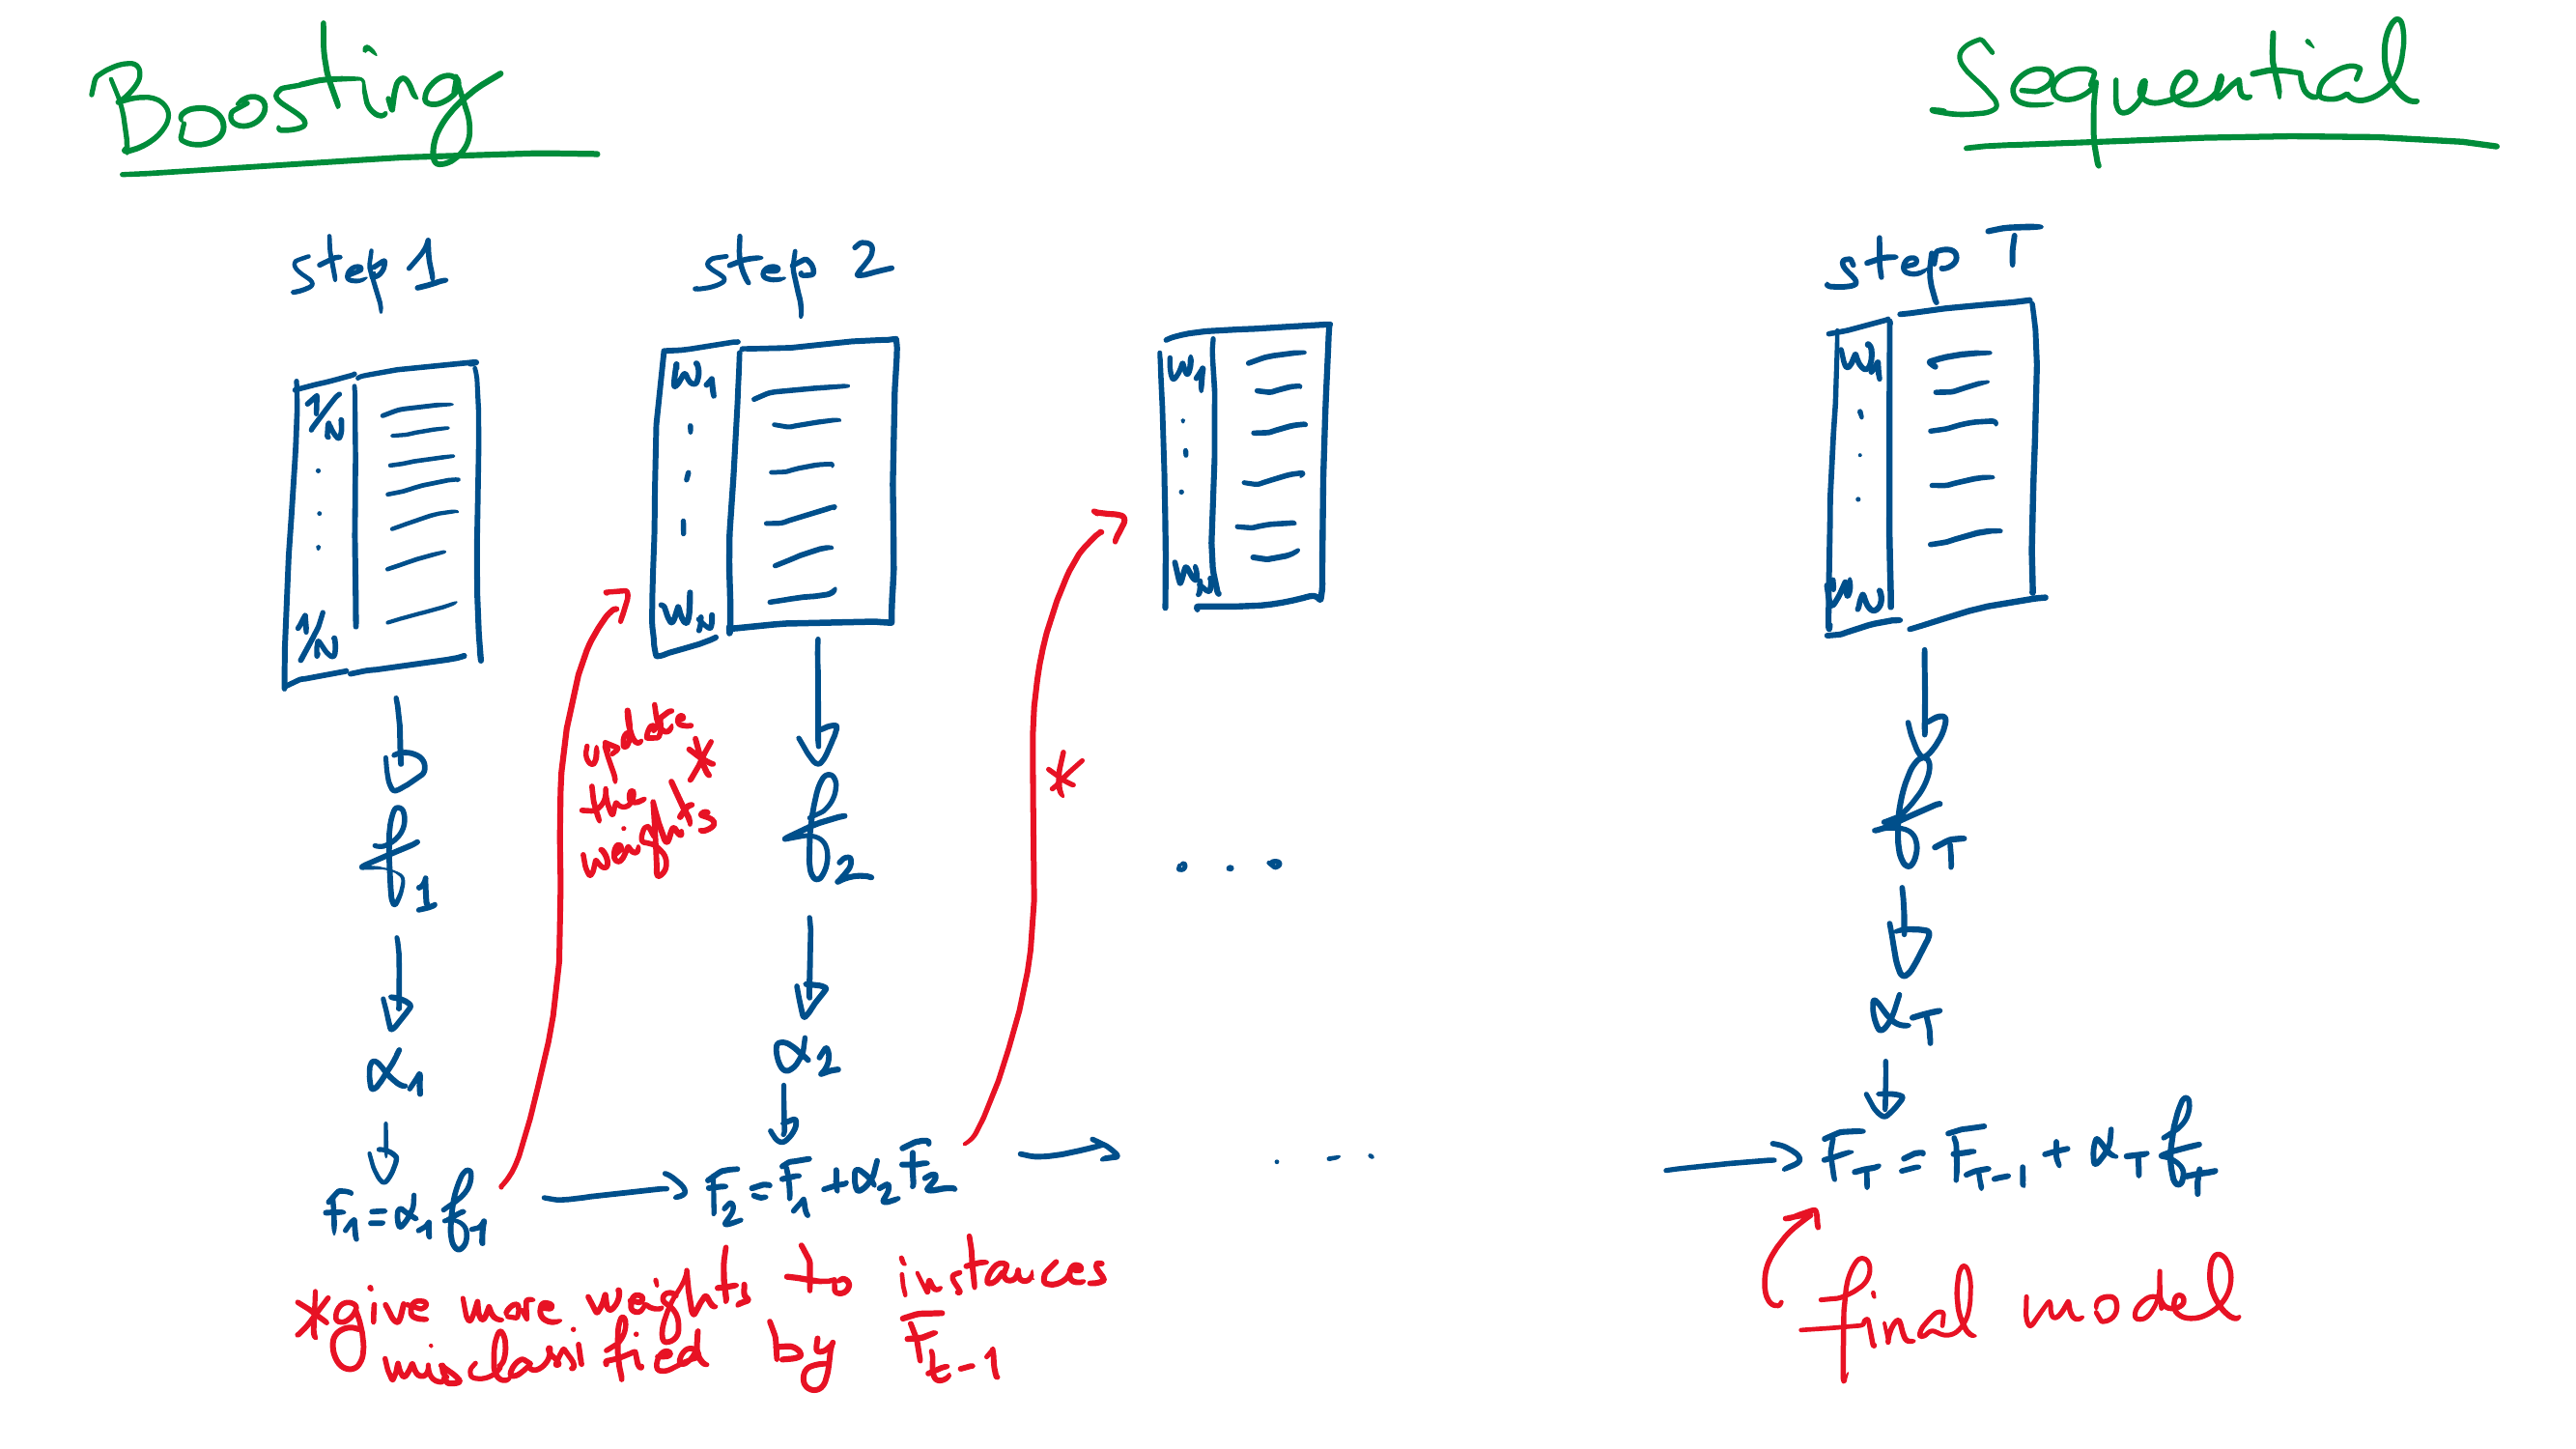
\includegraphics[width=13cm, page=1]{../Graphs/Bagging_Boosting_Illustrations.png}
\end{frame}
%%%%%%%%%%%%%%%%%%%%%%%%%%%%%
\begin{frame}
\frametitle{Bagging vs boosting}
\includegraphics[width=13cm, page=2]{../Graphs/Bagging_Boosting_Illustrations.png}
\end{frame}
%%%%%%%%%%%%%%%%%%%%%%%%%%%%%
%%%%%%%%%%%%%%%%%%%%%%%%%%%%%
\end{document}
%%%%%%%%%%%%%%%%%%%%%%%%%%%%%
%%%%%%%%%%%%%%%%%%%%%%%%%%%%%
\begin{frame}
\frametitle{Regression example}
Facebook data (see course on linear regression)
\begin{itemize}
\item Outcome $y$: {\tt Lifetime Post Consumers} - the number of people who clicked anywhere in a post.
\item The seven features are 
\begin{itemize}
\scriptsize
\item $x_1$: {\tt Page.total.likes} Number of people who have liked the company's page (!!page $\neq$ post).
\item $x_2$: {\tt Type} Type of content (Link, Photo, Status, Video)
\item $x_3$: {\tt Category} Manual content characterization: action (special offers and contests), product (direct advertisement, explicit brand content), and inspiration (non-explicit brand related content).
\item $x_4$: {\tt Post.Month} Month the post was published (January, February, March, ...,
December).
\item $x_5$: {\tt Post.Weekday} Weekday the post was published (Sunday, Monday, ...,
Saturday)
\item $x_6$: {\tt Post.Hour} Hour the post was published (0, 1, 2, 3, 4, ..., 23).
\item $x_7$: {\tt Paid} If the company paid to Facebook for advertising (yes, no).
\end{itemize}
\item There are 500 instances.
\end{itemize}
\end{frame}
%%%%%%%%%%%%%%%%%%%%%%%%%%%%%
\begin{frame}[fragile]
\frametitle{Regression example}
Below the result of a single tree and of a random forest (package {\tt ranger}).
\scriptsize
\begin{verbatim}
> FB.rp <- rpart(Lifetime.Post.Consumers ~ ., data=df.tr)
> RMSE(pred = predict(FB.rp, newdata = df.te), obs=df.te$Lifetime.Post.Consumers)
[1] 734.8711

> FB.rf <- ranger(Lifetime.Post.Consumers ~ ., data=df.tr, mtry=2)
> RMSE(pred = predict(FB.rf, data = df.te)$prediction, 
       + obs=df.te$Lifetime.Post.Consumers)                                                        $
[1] 632.0568
\end{verbatim}
\normalsize
\end{frame}
%%%%%%%%%%%%%%%%%%%%%%%%%%%%%
\begin{frame}[fragile]
\frametitle{Code examples with variable importance}
\scriptsize
In {\tt randomForest}:
\begin{verbatim}
iris.rf <- randomForest(Species~., data=iris.tr) 
varImpPlot(iris.rf) ## get variable importance
\end{verbatim}
In {\tt ranger}:
\begin{verbatim}
FB.rf <- ranger(Lifetime.Post.Consumers ~ ., data=df.tr, importance='impurity'))
importance(FB.rf) ## get variable importance
\end{verbatim}
In {\tt caret}, with {\tt train}:
\begin{verbatim}
FB.rf.tr <- train(Lifetime.Post.Consumers ~., data = df.tr, method = "ranger",
      trControl=trctrl, importance='impurity')			
varImp(FB.rf.tr)
\end{verbatim}
\end{frame}
%%%%%%%%%%%%%%%%%%%%%%%%%%%%%
\begin{frame}
\frametitle{Why does it work?}
What is the interest of selecting a random subset of features?\\
\vspace{0.3cm}
We have seen that a central reason of the efficiency of bagging was that the models predictions should be uncorrelated. Since all the models are in principle good, this non-correlation will bring stability to the final prediction.\\
\vspace{0.3cm}
For RF, a consequence of forcing the exclusion of some features in some splits in some models is that the range of features used in the final prediction is enlarged (compare to a global model that uses only few features). This gives more chance for extrapolation outside the training set.
\end{frame}
%%%%%%%%%%%%%%%%%%%%%%%%%%%%%
\begin{frame}
\frametitle{Why does it work?}
{\bf Example}: with the Boston data set, below are two small trees with features selected at random, with MSE's on the test set at 70.2 and 64.2.
\vspace{-1cm}
\begin{center}
\includegraphics[width=6cm]{SmallTree1.png}\\
\vspace{-3cm}
\includegraphics[width=6cm]{SmallTree2.png}
\end{center}
\end{frame}
%%%%%%%%%%%%%%%%%%%%%%%%%%%%%
\begin{frame}
\frametitle{Why does it work?}
The comparison of the predictions on the test set of the two trees gives
\begin{center}
\includegraphics[width=5cm]{SmallTreesPred.png}
\end{center}
The correlation between their predictions is 0.45. The one with the bagging trees was 0.89. That is, these models have a lower correlation due to feature random selection.
\end{frame}
%%%%%%%%%%%%%%%%%%%%%%%%%%%%%
\begin{frame}
\frametitle{Why does it work?}
Comparing the predictions with the observed values gives
\begin{center}
\includegraphics[width=5cm]{SmallTreesPredvsObs.png}
\end{center}
The averaging is important to bring stability in the predictions because of the size of the two trees.
\end{frame}
%%%%%%%%%%%%%%%%%%%%%%%%%%%%%
\begin{frame}
\frametitle{Why does it work?}
With the averages,
\begin{center}
\includegraphics[width=6cm]{SmallTreesPredvsObsAvg.png}
\end{center}
The MSE of the average is 60.44, lower than the MSE of each model (70.2 and 64.2).
\end{frame}
%%%%%%%%%%%%%%%%%%%%%%%%%%%%%
\begin{frame}
\frametitle{Why does it work?}
The procedure is now extended using function {\tt randomForest} of the eponymous package. It gives the following predictions, below compared to a single (pruned) regression tree:
\begin{center}
\includegraphics[width=5cm]{RFPred.png}
\end{center}
The MSE's are 26.9 (single tree) and 14.0 (RF).
\end{frame}
%%%%%%%%%%%%%%%%%%%%%%%%%%%%%
\begin{frame}
\frametitle{Variable importance}
Because they mix several trees, random forests lose all interpretation power. In particular, it is not easy to determine whether a given feature is important for the prediction.\\
\vspace{0.3cm}
The {\bf importance} of a variable can be evaluated by:
\begin{itemize}
\item In the test set, shuffle the variable instances.
\item Pass the test set to the learner to compute the predictions
\item Check the prediction quality (RMSE, Accuracy, ...).
\item If the variable is important, giving to the model an incorrect value of this variable should decrease a lot the prediction quality. 
\item Repeat for all the variables.
\end{itemize}
\end{frame}
%%%%%%%%%%%%%%%%%%%%%%%%%%%%%
\begin{frame}
\frametitle{Variable importance: illustration}
\begin{center}
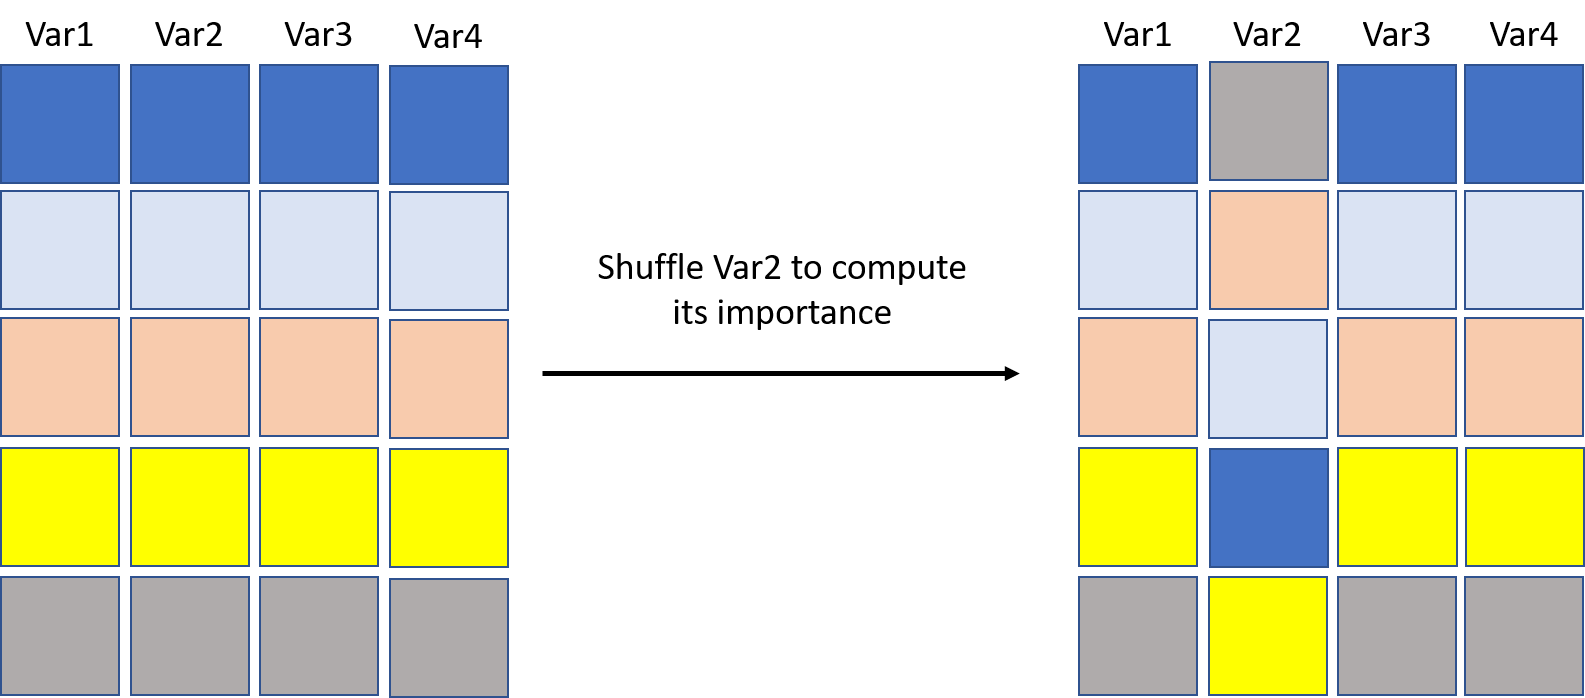
\includegraphics[width=10cm]{VI_Illustr.png}
\end{center}
If predictions using the right-hand side data are the same as the left-hand side ones, the Var2 is not important.
\end{frame}
%%%%%%%%%%%%%%%%%%%%%%%%%%%%%
\begin{frame}
\frametitle{Variable importance}
{\bf Example}: with the Boston data set, below is the tree on a training set of 380 instances (after pruning). Its MSE on the test set is 34.42.
\begin{center}
\includegraphics[width=6cm]{Boston_RT.png}
\end{center}
\end{frame}
%%%%%%%%%%%%%%%%%%%%%%%%%%%%%
\begin{frame}
\frametitle{Variable importance}
Now, in the test set, the variable {\tt lstat} is shuffled at random. The MSE on the new test set is 63.62. 
\begin{center}
\includegraphics[width=8cm]{Boston_RT_shufflstat.png}
\end{center}
Going from RMSE=34.42 to RMSE=63.62 looks like a substantial increase. Variable {\tt lstat} is important.
\end{frame}
%%%%%%%%%%%%%%%%%%%%%%%%%%%%%
\begin{frame}
\frametitle{Variable importance}
The experience is now repeated with variable {\tt zn}. The MSE on the new test set is 34.42 (i.e. the same as when {\tt zn} is not shuffled). 
\begin{center}
\includegraphics[width=8cm]{Boston_RT_shuffzn.png}
\end{center}
Since the RMSE is unchanged when variable {\tt zn} is perturbed, this variable is not important for the prediction. This is not surprising since {\tt zn} is not used by the model. 
\end{frame}
%%%%%%%%%%%%%%%%%%%%%%%%%%%%%
%\begin{frame}
%\frametitle{Variable importance}
%Repeating with variable {\tt age}. The MSE on the new test set is still 34.42. 
%\begin{center}
%\includegraphics[width=8cm]{Boston_RT_shuffage.png}
%\end{center}
%Even if used by the model, {\tt age} is not an important variable. 
%\end{frame}
%%%%%%%%%%%%%%%%%%%%%%%%%%%%%
\begin{frame}
\frametitle{Variable importance}
This approach can be adapted to random forests. For each sub-tree, a subset was sampled with replacement from the original training set. It means that there are instances that are in the original training set but not in the subset. They are the {\bf out-of-bag} (OOB) instances. \\
\vspace{0.3cm}
The importance is computed on the OOB, in each tree: for each feature, 
\begin{itemize}
\item Shuffle the feature column of the OOB set
\item Measure the relative increase of the MSE following this operation when using the model to predict the OOB.
\end{itemize}
This is repeated for all the models. For each feature, the average increase of the MSE over all the trees is computed. They are represented on a graph.
\end{frame}
%%%%%%%%%%%%%%%%%%%%%%%%%%%%%
\begin{frame}
\frametitle{Variable importance}
\begin{center}
\includegraphics[width=6cm]{Boston_RT_VI1.png}
\end{center}
The above method is called the {\bf permutation measure}. For classification, the Gini index replaces the MSE. Any other score could be used in theory.
\end{frame}
%%%%%%%%%%%%%%%%%%%%%%%%%%%%%
\begin{frame}
\frametitle{Variable importance}
Another computation of the importance is by measuring the average increase in the node purity each time a feature is used in a split. The average is taken over all the splits and all the trees. 
\begin{center}
\includegraphics[width=6cm]{Boston_RT_VI2.png}
\end{center}
\end{frame}
%%%%%%%%%%%%%%%%%%%%%%%%%%%%%
%%%%%%%%%%%%%%%%%%%%%%%%%%%%%
\end{document}

%%%%%%%%%%%%%%%%%%%%%%%%%%%%%
%%%%%%%%%%%%%%%%%%%%%%%%%%%%%
%%%%%%%%%%%%%%%%%%%%%%%%%%%%%
%%%%%%%%%%%%%%%%%%%%%%%%%%%%%
%%%%%%%%%%%%%%%%%%%%%%%%%%%%%
%%%%%%%%%%%%%%%%%%%%%%%%%%%%%
%%%%%%%%%%%%%%%%%%%%%%%%%%%%%
%%%%%%%%%%%%%%%%%%%%%%%%%%%%%
%%%%%%%%%%%%%%%%%%%%%%%%%%%%%
%%%%%%%%%%%%%%%%%%%%%%%%%%%%%
\begin{frame}
\frametitle{Bagging}
{\bf Example}: Reviewing the Facebook data (see linear regression). We predict {\tt Lifetime.Post.Consumers} from the other 13 features using a linear regression. The full model (all features) overfits the data. With a bag of 150 models, the overfitting is reduced without loosing too much accuracy.
\begin{center}
\begin{tabular}{c|c|c|}
RMSE & Training set ($90\%$)& Test set ($10\%$)\\
\hline
Full model & 32.02 & 41.75\\ 
\hline
Bag of 150 models & 33.21 & 34.05\\ 
\hline
\end{tabular}
\end{center}
\end{frame}
%%%%%%%%%%%%%%%%%%%%%%%%%%%%%
\begin{frame}[fragile]
\frametitle{Bagging}
\tiny
\begin{verbatim}
## Full model
fb.lm <- lm(Lifetime.Post.Consumers~., data=facebook.tr, na.action = na.exclude)
fb.pred <- predict(fb.lm, newdata = facebook.te)
(RMSE <- sqrt(mean((fb.pred - facebook.te$Lifetime.Post.Consumers)^2, na.rm=TRUE)))
(RMSE.app <- sqrt(mean((facebook.tr$Lifetime.Post.Consumers - predict(fb.lm))^2, na.rm=TRUE)))

## Bagging
nModels <- 150
fb.lmbag <- list()
fb.bag.pred.te <- 0
fb.bag.pred.tr <- 0
for (j in 1:nModels){
  index <- sample(1:nrow(facebook.tr), size=nrow(facebook.tr), replace=TRUE)
  fb.lmbag[[j]] <- lm(Lifetime.Post.Consumers~., data=facebook.tr[index,])
  fb.bag.pred.te <- fb.bag.pred.te + predict(fb.lmbag[[j]], newdata = facebook.te)
  fb.bag.pred.tr <- fb.bag.pred.tr + predict(fb.lmbag[[j]], newdata = facebook.tr)
}
fb.bag.pred.te <- fb.bag.pred.te / nModels
fb.bag.pred.tr <- fb.bag.pred.tr / nModels
(RMSE.bag.te <- sqrt(mean((fb.bag.pred.te - facebook.te$Lifetime.Post.Consumers)^2, na.rm=TRUE)))
(RMSE.bag.tr <- sqrt(mean((fb.bag.pred.tr - facebook.tr$Lifetime.Post.Consumers)^2, na.rm=TRUE)))
\end{verbatim}
\end{frame}
%%%%%%%%%%%%%%%%%%%%%%%%%%%%%
